\documentclass[]{article}
\usepackage{lmodern}
\usepackage{amssymb,amsmath}
\usepackage{ifxetex,ifluatex}
\usepackage{fixltx2e} % provides \textsubscript
\ifnum 0\ifxetex 1\fi\ifluatex 1\fi=0 % if pdftex
  \usepackage[T1]{fontenc}
  \usepackage[utf8]{inputenc}
\else % if luatex or xelatex
  \ifxetex
    \usepackage{mathspec}
  \else
    \usepackage{fontspec}
  \fi
  \defaultfontfeatures{Ligatures=TeX,Scale=MatchLowercase}
\fi
% use upquote if available, for straight quotes in verbatim environments
\IfFileExists{upquote.sty}{\usepackage{upquote}}{}
% use microtype if available
\IfFileExists{microtype.sty}{%
\usepackage{microtype}
\UseMicrotypeSet[protrusion]{basicmath} % disable protrusion for tt fonts
}{}
\usepackage[margin=1in]{geometry}
\usepackage{hyperref}
\PassOptionsToPackage{usenames,dvipsnames}{color} % color is loaded by hyperref
\hypersetup{unicode=true,
            pdftitle={The Aerial Parking Lot dataset: A description},
            pdfauthor={Nisim Hurst},
            colorlinks=true,
            linkcolor=Maroon,
            citecolor=Blue,
            urlcolor=blue,
            breaklinks=true}
\urlstyle{same}  % don't use monospace font for urls
\usepackage{color}
\usepackage{fancyvrb}
\newcommand{\VerbBar}{|}
\newcommand{\VERB}{\Verb[commandchars=\\\{\}]}
\DefineVerbatimEnvironment{Highlighting}{Verbatim}{commandchars=\\\{\}}
% Add ',fontsize=\small' for more characters per line
\usepackage{framed}
\definecolor{shadecolor}{RGB}{248,248,248}
\newenvironment{Shaded}{\begin{snugshade}}{\end{snugshade}}
\newcommand{\AlertTok}[1]{\textcolor[rgb]{0.94,0.16,0.16}{#1}}
\newcommand{\AnnotationTok}[1]{\textcolor[rgb]{0.56,0.35,0.01}{\textbf{\textit{#1}}}}
\newcommand{\AttributeTok}[1]{\textcolor[rgb]{0.77,0.63,0.00}{#1}}
\newcommand{\BaseNTok}[1]{\textcolor[rgb]{0.00,0.00,0.81}{#1}}
\newcommand{\BuiltInTok}[1]{#1}
\newcommand{\CharTok}[1]{\textcolor[rgb]{0.31,0.60,0.02}{#1}}
\newcommand{\CommentTok}[1]{\textcolor[rgb]{0.56,0.35,0.01}{\textit{#1}}}
\newcommand{\CommentVarTok}[1]{\textcolor[rgb]{0.56,0.35,0.01}{\textbf{\textit{#1}}}}
\newcommand{\ConstantTok}[1]{\textcolor[rgb]{0.00,0.00,0.00}{#1}}
\newcommand{\ControlFlowTok}[1]{\textcolor[rgb]{0.13,0.29,0.53}{\textbf{#1}}}
\newcommand{\DataTypeTok}[1]{\textcolor[rgb]{0.13,0.29,0.53}{#1}}
\newcommand{\DecValTok}[1]{\textcolor[rgb]{0.00,0.00,0.81}{#1}}
\newcommand{\DocumentationTok}[1]{\textcolor[rgb]{0.56,0.35,0.01}{\textbf{\textit{#1}}}}
\newcommand{\ErrorTok}[1]{\textcolor[rgb]{0.64,0.00,0.00}{\textbf{#1}}}
\newcommand{\ExtensionTok}[1]{#1}
\newcommand{\FloatTok}[1]{\textcolor[rgb]{0.00,0.00,0.81}{#1}}
\newcommand{\FunctionTok}[1]{\textcolor[rgb]{0.00,0.00,0.00}{#1}}
\newcommand{\ImportTok}[1]{#1}
\newcommand{\InformationTok}[1]{\textcolor[rgb]{0.56,0.35,0.01}{\textbf{\textit{#1}}}}
\newcommand{\KeywordTok}[1]{\textcolor[rgb]{0.13,0.29,0.53}{\textbf{#1}}}
\newcommand{\NormalTok}[1]{#1}
\newcommand{\OperatorTok}[1]{\textcolor[rgb]{0.81,0.36,0.00}{\textbf{#1}}}
\newcommand{\OtherTok}[1]{\textcolor[rgb]{0.56,0.35,0.01}{#1}}
\newcommand{\PreprocessorTok}[1]{\textcolor[rgb]{0.56,0.35,0.01}{\textit{#1}}}
\newcommand{\RegionMarkerTok}[1]{#1}
\newcommand{\SpecialCharTok}[1]{\textcolor[rgb]{0.00,0.00,0.00}{#1}}
\newcommand{\SpecialStringTok}[1]{\textcolor[rgb]{0.31,0.60,0.02}{#1}}
\newcommand{\StringTok}[1]{\textcolor[rgb]{0.31,0.60,0.02}{#1}}
\newcommand{\VariableTok}[1]{\textcolor[rgb]{0.00,0.00,0.00}{#1}}
\newcommand{\VerbatimStringTok}[1]{\textcolor[rgb]{0.31,0.60,0.02}{#1}}
\newcommand{\WarningTok}[1]{\textcolor[rgb]{0.56,0.35,0.01}{\textbf{\textit{#1}}}}
\usepackage{longtable,booktabs}
\usepackage{graphicx,grffile}
\makeatletter
\def\maxwidth{\ifdim\Gin@nat@width>\linewidth\linewidth\else\Gin@nat@width\fi}
\def\maxheight{\ifdim\Gin@nat@height>\textheight\textheight\else\Gin@nat@height\fi}
\makeatother
% Scale images if necessary, so that they will not overflow the page
% margins by default, and it is still possible to overwrite the defaults
% using explicit options in \includegraphics[width, height, ...]{}
\setkeys{Gin}{width=\maxwidth,height=\maxheight,keepaspectratio}
\IfFileExists{parskip.sty}{%
\usepackage{parskip}
}{% else
\setlength{\parindent}{0pt}
\setlength{\parskip}{6pt plus 2pt minus 1pt}
}
\setlength{\emergencystretch}{3em}  % prevent overfull lines
\providecommand{\tightlist}{%
  \setlength{\itemsep}{0pt}\setlength{\parskip}{0pt}}
\setcounter{secnumdepth}{0}
% Redefines (sub)paragraphs to behave more like sections
\ifx\paragraph\undefined\else
\let\oldparagraph\paragraph
\renewcommand{\paragraph}[1]{\oldparagraph{#1}\mbox{}}
\fi
\ifx\subparagraph\undefined\else
\let\oldsubparagraph\subparagraph
\renewcommand{\subparagraph}[1]{\oldsubparagraph{#1}\mbox{}}
\fi

%%% Use protect on footnotes to avoid problems with footnotes in titles
\let\rmarkdownfootnote\footnote%
\def\footnote{\protect\rmarkdownfootnote}

%%% Change title format to be more compact
\usepackage{titling}

% Create subtitle command for use in maketitle
\newcommand{\subtitle}[1]{
  \posttitle{
    \begin{center}\large#1\end{center}
    }
}

\setlength{\droptitle}{-2em}
  \title{The Aerial Parking Lot dataset: A description}
  \pretitle{\vspace{\droptitle}\centering\huge}
  \posttitle{\par}
  \author{\href{mailto:langheran@gmail.com}{Nisim Hurst}}
  \preauthor{\centering\large\emph}
  \postauthor{\par}
  \predate{\centering\large\emph}
  \postdate{\par}
  \date{Thursday 26 July 2018}

\usepackage{float}
\usepackage{caption}
\usepackage{listings}
\usepackage{attachfile}
\makeatletter\renewcommand*{\fps@figure}{H}\makeatother

\usepackage{amsthm}
\newtheorem{theorem}{Theorem}
\newtheorem{lemma}{Lemma}
\theoremstyle{definition}
\newtheorem{definition}{Definition}
\newtheorem{corollary}{Corollary}
\newtheorem{proposition}{Proposition}
\theoremstyle{definition}
\newtheorem{example}{Example}
\theoremstyle{definition}
\newtheorem{exercise}{Exercise}
\theoremstyle{remark}
\newtheorem*{remark}{Remark}
\newtheorem*{solution}{Solution}
\begin{document}
\maketitle
\begin{abstract}
The Aerial Parking Space dataset (\emph{APKLOT}) is intended for two
audiences: algorithm designers and researchers who want to validate the
state of the art measured by performance on the Parking Space dataset.
\end{abstract}

{
\hypersetup{linkcolor=black}
\setcounter{tocdepth}{5}
\tableofcontents
}
\hypertarget{introduction}{%
\subsection{Introduction}\label{introduction}}

The main goal of this dataset is to segment parking spot spaces from
several parking lots of the world in realistic satellite photos.
Satellite photos were generated using the free Google Maps API service.
Given a training set, this is fundamentally a supervised-learning
learning problem.

For the purpose of this dataset, a parking spot is a painted area
specially designed inside the parking lot for parking. we are not
considering the following:

\begin{itemize}
\tightlist
\item
  Parking spots outside the parking lot.
\item
  Badly parked vehicles, including those parked on the traffic lane and
  non-parking spot (benches, gardens, etc).
\item
  Debris or machinery in the parking spot when it is used as manner of
  storage facility.
\item
  Trees in the way of the parking spot.
\end{itemize}

These are the countries and cities included in \emph{APKLOT}:

\begin{longtable}[]{@{}lll@{}}
\caption{Countries and cities included in \emph{APKLOT}}\tabularnewline
\toprule
Country & City & \# Instances\tabularnewline
\midrule
\endfirsthead
\toprule
Country & City & \# Instances\tabularnewline
\midrule
\endhead
México & México & 90\tabularnewline
México & Monterrey & 6\tabularnewline
México & Guadalajara & 7\tabularnewline
United States & New York & 119\tabularnewline
United States & Los Ángeles & 78\tabularnewline
United States & Chicago & 25\tabularnewline
United States & Houston & 53\tabularnewline
Chile & Santiago & 62\tabularnewline
Spain & Madrid & 23\tabularnewline
Japan & Tokyo & 40\tabularnewline
\bottomrule
\end{longtable}

\hypertarget{objectives}{%
\subsection{Objectives}\label{objectives}}

\begin{itemize}
\tightlist
\item
  Provides aerial view image dataset for parking spot segmentation,
  i.e.~generate pixel-wise areas given the class visible at each pixel
  through a mask.
\item
  Provides benchmark code for evaluating the quality of the masks.
\item
  Enables evaluation and comparison of different methods vs the results
  of obtained in the companion paper.
\end{itemize}

\hypertarget{related-work}{%
\subsection{Related work}\label{related-work}}

The authors on
{[}\protect\hyperlink{ref-DBLP:journalsux2fcorrux2fHsiehLH17}{1}{]}
present the CARPK dataset. It is the first large-scale dataset for
counting cars from flying drones. CARPK provides 89,777 instances
bounding boxes from moving video in 4 distinct parking lots.

\hypertarget{ground-truth-description}{%
\subsection{Ground truth description}\label{ground-truth-description}}

The ground truth is available in two formats:

\begin{enumerate}
\def\labelenumi{\arabic{enumi}.}
\tightlist
\item
  \textbf{Pascal VOC 2010.} The PASCAL Visual Object Classes format
  {[}\protect\hyperlink{ref-Everingham10}{2}{]} is one of the most used
  for segmentation. Here is a brief description of the each folder,
  however if you wish to dive deeper you can refer to
  \href{http://host.robots.ox.ac.uk/pascal/VOC/}{the Pascal VOC page}:

  \begin{enumerate}
  \def\labelenumii{\arabic{enumii}.}
  \tightlist
  \item
    \textbf{JPEGImages.} The binary image files on JPEG compression
    format are stored here.
  \item
    \textbf{Annotations.} Contains xml Pascal VOC annotation files. The
    most prominent feature of these files is that they do not contain
    the real shape polygon, just a bounding rectangle without
    orientation.
  \item
    \textbf{ImageSets\textbackslash{}Segmentation.} 3 text files are
    included here: (1) train.txt, (2) trainval.txt and (3) val.txt. Each
    is a list of files without extension for the train, validation and
    test set respectively.
  \item
    \textbf{SegmentationClass.} Contains the masks for training by class
    i.e.~a class-wise color is assigned.
  \item
    \textbf{SegmentationObject.} Contains the masks i.e.~a object-wise
    color is assigned. Due we are using just one class, it is worthwhile
    to point out that this folder contains exactly the same images as
    the \textbf{SegmentationClass} folder and is included for
    compatibility issues.
  \end{enumerate}
\end{enumerate}

\begin{figure}

{\centering 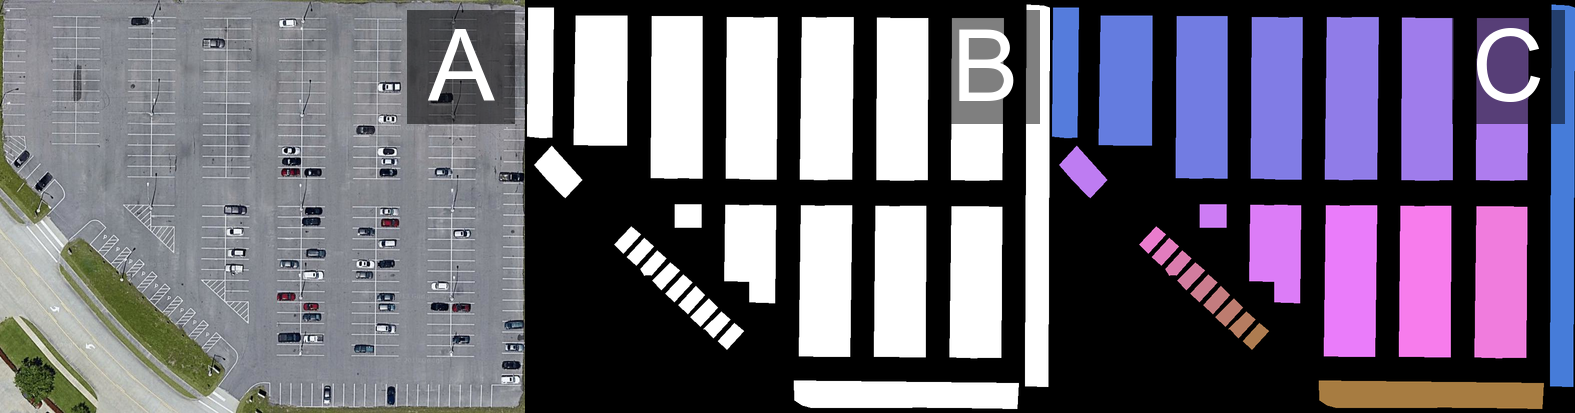
\includegraphics[width=0.45\linewidth]{images/apklot_examples/seg} 

}

\caption{Example segmentation images on the Pascal VOC: (A) \textbf{JPEGImages} folder, (B) \textbf{SegmentationClass} folder, (C) \textbf{SegmentationObject} folder. }\label{fig:fig1}
\end{figure}

\begin{enumerate}
\def\labelenumi{\arabic{enumi}.}
\setcounter{enumi}{1}
\tightlist
\item
  \textbf{LabelMe masks.} LabelMe mask format was introduced as part of
  a \href{http://labelme.csail.mit.edu/Release3.0/}{web site} for image
  segmentation on
  {[}\protect\hyperlink{ref-DBLP:journalsux2fcorrux2fabs-1210-3448}{3}{]}.
  Here are the most important elements of the ensued json file:

  \begin{enumerate}
  \def\labelenumii{\arabic{enumii}.}
  \tightlist
  \item
    \textbf{shapes.} An array containing each of the shape polygons that
    were labeled as a parking spot.
  \item
    \textbf{imageData.} This element was deleted on behalf of reducing
    redundancy and making the dataset smaller. There is one Jupyter
    Notebook on the \textbf{labelme} folder - \emph{imagedata.ipynb} -
    which can restore or delete this dictionary element if one would
    like to modify some area mapping with the
    \href{https://github.com/wkentaro/labelme}{labelme python} tool. You
    should restore the imageData dictionary element in order to run once
    again the labelme tool on the provided json file.
  \item
    \textbf{Other features.} lineColor, fillColor and image path is also
    provided for the \emph{labelme} tool to render the polygons on edit
    mode.
  \end{enumerate}
\end{enumerate}

\hypertarget{included-scripts-guide}{%
\subsection{Included scripts guide}\label{included-scripts-guide}}

All the scripts were written in Jupyter Notebooks with a python 3.6
kernel for readers' ease. The scripts and the folder that contains them
are numbered for you to execute in order on behalf of achieving the
following objectives:

\begin{enumerate}
\def\labelenumi{\arabic{enumi}.}
\tightlist
\item
  Select the train, validation and tests sets for building the PASCAL
  dataset from the labelme annotations.
\item
  Generate each of the required folders for the PASCAL VOC 2010 format.
\item
  Expand the image set with jittering and corresponding annotations.
\item
  Extract statistical features to evaluate the datasets
\end{enumerate}

\begin{verbatim}

                         +---1. build_training_test_folders
                         |   |   build.ipynb
                         |   \---builds
                         |       \---\<date\>
                         +---2. pascal
                         |   |   1. JPEGImages.ipynb
                         |   |   2. Annotations.ipynb
                         |   |   3. ImageSets.Segmentation.ipynb
                         |   |   4. SegmentationClass.ipynb
                         |   \---5. SegmentationObject.ipynb
                         +---3. jittering
                         |   |   1. Jittering.ipynb
                         |   |   2. Annotations.ipynb
                         |   |   3. ImageSets.Segmentation.ipynb
                         |   \---4. MoveEmpty.ipynb
                         \---4. features
                             |   1. marked_area.ipynb
                             |   2. stats features.ipynb
                             \---3. evaluation.ipynb
\end{verbatim}

\normalsize
\begin{figure}
\captionof{lstlisting}{Included scripts tree file structure}
\end{figure}

\hypertarget{format-conversion}{%
\subsection{Format conversion}\label{format-conversion}}

\hypertarget{subset-selection---1.-build_training_test_folders}{%
\subsubsection{\texorpdfstring{Subset selection -
\texttt{1.\ build\_training\_test\_folders}}{Subset selection - 1. build\_training\_test\_folders}}\label{subset-selection---1.-build_training_test_folders}}

Sometimes it is convenient to just reduce the training data for
selecting the sample size or filter out some countries we want to
ignore. In those cases having a script to rebuild the dataset is
convenient.

That said, the purpose of this task is to allow change the training and
test sets from all the images folder and two txt files that specify both
training and testing filenames without extension. Thus, the input is the
images folder containing both png images and json labelme annotations
and two txt files list. The output is two folders containing those
images. Subset selection is done in this folder, \emph{1.
build\_training\_test\_folders}. Inside you will find \emph{build.ipynb}
notebook. You have to setup the following:

\begin{enumerate}
\def\labelenumi{\arabic{enumi}.}
\tightlist
\item
  \textbf{training.txt} and \textbf{testing.txt} files.
\item
  Inside the script:

  \begin{enumerate}
  \def\labelenumii{\arabic{enumii}.}
  \tightlist
  \item
    \textbf{IMAGES\_PATH.} Where are all the png images and labelme
    annotations located.
  \item
    \textbf{BUILD\_DAY.} The name of the folder where the
    \textbf{training.txt} and \textbf{testing.txt} files are.
  \item
    \textbf{BUILD\_OUTPUT.} Where the \textbf{training} and
    \textbf{testing} folders will be created for the new dataset.
  \end{enumerate}
\end{enumerate}

Then, you can just run the script and the folders will be generated at
the desired location.

\hypertarget{pascal-format-conversion---2.-pascal}{%
\subsubsection{\texorpdfstring{Pascal format conversion -
\texttt{2.\ pascal}}{Pascal format conversion - 2. pascal}}\label{pascal-format-conversion---2.-pascal}}

\hypertarget{statistical-features---4.-features}{%
\subsection{\texorpdfstring{Statistical features -
\texttt{4.\ features}}{Statistical features - 4. features}}\label{statistical-features---4.-features}}

Finally, we want to assess how well suited is the data by itself to an
specific algorithm we are developing. E.g., in some environments we
would like to filter out parking spaces with very little annotated
spaces to train more effectively, in others we would like to bound the
algorithm in terms of computational power.

\begin{figure}

{\centering 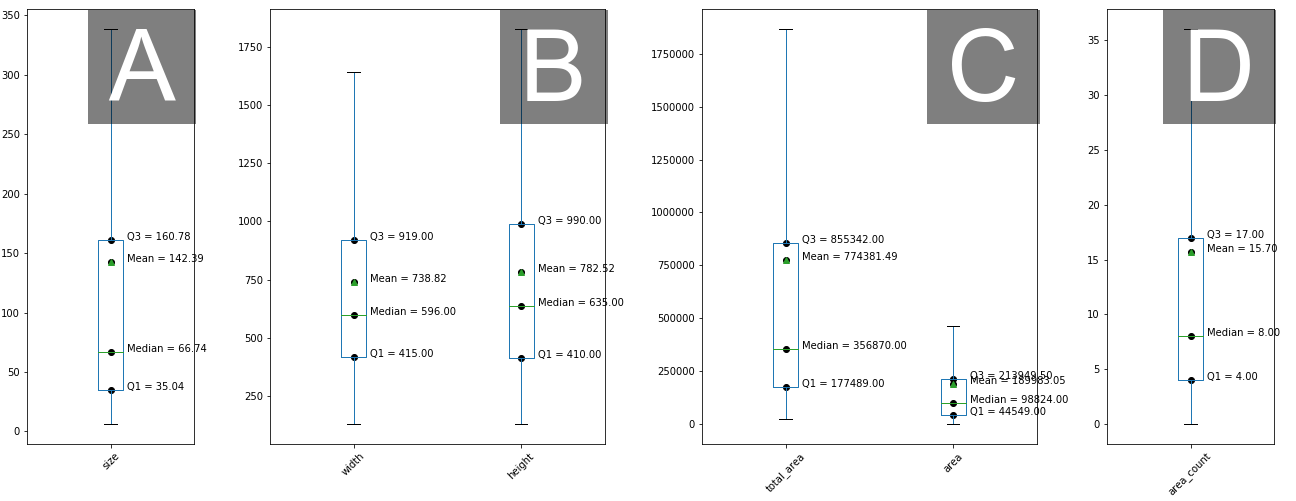
\includegraphics[width=0.9\linewidth]{images/features} 

}

\caption{Stats features from the APKLOT dataset: (A) size in KB, (B) width and height of the image, (C) total area vs annotated area, (D) area count per image. }\label{fig:fig2}
\end{figure}

Figure \ref{fig:fig2} show some of the statistical features that were
extracted by using the \emph{features.ipynb} script:

\begin{itemize}
\tightlist
\item
  \textbf{(A) Size.} We can see that the interquatile range lies beneath
  200KB. However, there maybe outliers reaching at most 3.4 MB. You
  should be careful in identifying these outliers in case your algorithm
  fall short of GPU memory.\footnote{By ignoring this warning and if you
    are using CUDA, a cudaMalloc error could be thrown.}
\end{itemize}

\begin{itemize}
\item
  \textbf{(B) Width and Height.} We can see from theses section that
  most images have a quadratic proportion with more or less the same
  width than height. Just as the previous case, a researcher could
  filter out images out of proportion to cope with the required input
  dimensions, e.g.~the input layer of a neural network.
\item
  \textbf{(C) Total area vs Annotated area.} This plot evince that
  sparse annotations dominate the dataset. Subset of a larger proportion
  could be assembled. However, we should take into account that the
  total area will ever be greater than the annotated area, and that due
  to the image borders will be approximately \(\frac{1}{4}\) of the
  \href{http://www.eveandersson.com/pi/monte-carlo-circle}{total}.
\item
  \textbf{(D) Area count per image.} We can see that each image has
  marked about \(15\) disconnected parking spot regions. There are
  images in which this number is really small, meaning a big fully
  connected clustered region. Depending on the problem, these regions
  might be desirable or just as well should be avoided. E.g. If we want
  to boost our segmentation algorithm with the prior probability from
  near regions, then big clusters should be used for training. On the
  contrary, if we want our algorithm to be robust enough to be able to
  detect parking spots solely on the appearance of just one of them,
  then images with a large area count (disconnected spots) should be
  selected.
\end{itemize}

\hypertarget{mask-evaluation}{%
\subsection{Mask evaluation}\label{mask-evaluation}}

\emph{3. evaluation.ipynb}

Intersection over union is an evaluation metric that is used extensively
on the object detection task, specifically in the PASCAL VOC dataset. It
is also known as the Jaccard index and measures the similarity pixel
sets between bounding boxes. The formula for calculating the
intersection over union o a bounding box is given by the following
formula: \[
\frac{iTP}{(iTP+FP+iFN)}
\]

\begin{figure}

{\centering 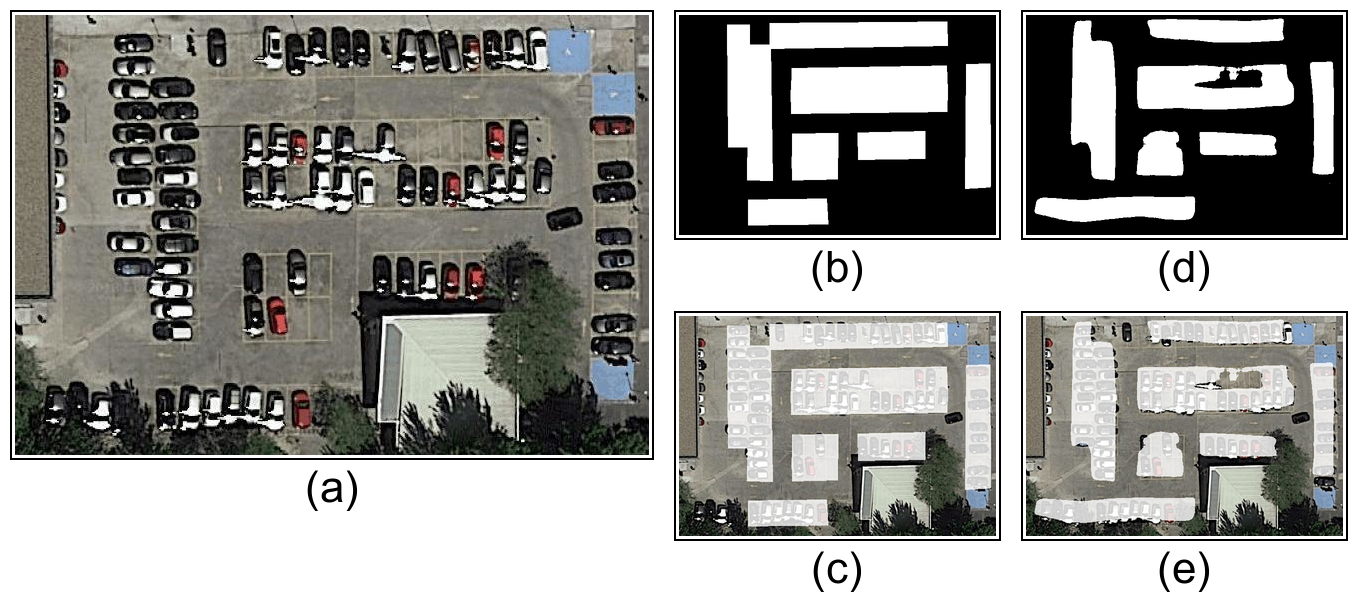
\includegraphics[width=0.65\linewidth]{images/segmentation_examples/seg} 

}

\caption{Example segmentation images on our dataset \emph{APKLOT}. }\label{fig:fig3}
\end{figure}

Clear metrics {[}\protect\hyperlink{ref-stiefelhagen2006clear}{4}{]}.

\hypertarget{dataset-expansion}{%
\subsection{Dataset expansion}\label{dataset-expansion}}

\hypertarget{download-more-images}{%
\subsubsection{Download more images}\label{download-more-images}}

\hypertarget{jittering---3.-jittering}{%
\subsubsection{\texorpdfstring{Jittering -
\texttt{3.\ jittering}}{Jittering - 3. jittering}}\label{jittering---3.-jittering}}

Jittering was done by using the
\href{https://github.com/aleju/imgaug}{imgaug} python library. The
following listing shows the code that was used for jittering:

\hypertarget{lst3}{%
\label{lst3}}%
\begin{Shaded}
\begin{Highlighting}[]
\NormalTok{seq }\OperatorTok{=}\NormalTok{ iaa.Sequential([}
\NormalTok{        iaa.Crop(px}\OperatorTok{=}\NormalTok{(}\DecValTok{0}\NormalTok{, }\DecValTok{50}\NormalTok{)), }\CommentTok{# crop images from each side by 0 to 16px (randomly chosen)}
\NormalTok{        iaa.Fliplr(}\FloatTok{0.5}\NormalTok{), }\CommentTok{# horizontally flip 50% of the images}
\NormalTok{        iaa.Flipud(}\FloatTok{0.5}\NormalTok{),}
\NormalTok{        iaa.Affine(rotate}\OperatorTok{=}\NormalTok{(}\OperatorTok{-}\DecValTok{45}\NormalTok{, }\DecValTok{45}\NormalTok{))}
\NormalTok{    ])}
\end{Highlighting}
\end{Shaded}

\normalsize
\begin{figure}
\captionof{lstlisting}{Jittering transformations}
\end{figure}

Lets give it a closer look and explain it line by line:

\begin{quote}
\begin{enumerate}
\def\labelenumi{(\arabic{enumi})}
\setcounter{enumi}{1}
\tightlist
\item
  Randomly crop by a value between 0 and 50 pixels
\item
  Horizontally flip 50\% of the images
\item
  Vertically flip 50\% of the images
\item
  Rotate images by a value between -45 and 45 degrees
\end{enumerate}
\end{quote}

\hypertarget{useful-software}{%
\subsection{Useful Software}\label{useful-software}}

\hypertarget{google-maps-api}{%
\subsubsection{Google Maps Api}\label{google-maps-api}}

\hypertarget{labelme}{%
\subsubsection{labelme}\label{labelme}}

We already digressed around labelme but here we indulge in a more formal
introduction. Labelme is a polygon manual annotation tool for
segmentation that was published on
{[}\protect\hyperlink{ref-DBLP:journalsux2fcorrux2fabs-1210-3448}{3}{]}.
It was first exposed to the public through a
\href{http://labelme.csail.mit.edu/Release3.0/}{webpage} and then
through a python pip
\href{https://github.com/wkentaro/labelme}{package}.

\hypertarget{dlib}{%
\subsubsection{dlib}\label{dlib}}

Dlib is an open source library that was published on
{[}\protect\hyperlink{ref-King:2009:DML:1577069.1755843}{5}{]}. It has
extensive documentation through its \href{http://dlib.net/}{webpage}.

\hypertarget{history-and-background}{%
\subsection{History and Background}\label{history-and-background}}

\begin{longtable}[]{@{}llll@{}}
\toprule
\begin{minipage}[b]{0.02\columnwidth}\raggedright
Year\strut
\end{minipage} & \begin{minipage}[b]{0.42\columnwidth}\raggedright
Statistics\strut
\end{minipage} & \begin{minipage}[b]{0.24\columnwidth}\raggedright
New developments\strut
\end{minipage} & \begin{minipage}[b]{0.20\columnwidth}\raggedright
Notes\strut
\end{minipage}\tabularnewline
\midrule
\endhead
\begin{minipage}[t]{0.02\columnwidth}\raggedright
2018\strut
\end{minipage} & \begin{minipage}[t]{0.42\columnwidth}\raggedright
Only 1 class discriminating between parking spot and other spaces.
\linebreak Train: \linebreak \hspace*{1cm} \(300\) images
\linebreak \hspace*{1cm} \(4034\) labelme polygons
\linebreak Validation: \linebreak \hspace*{1cm} \(100\) images
\linebreak \hspace*{1cm} \(1513\) labelme polygons \linebreak Test:
\linebreak \hspace*{1cm} \(101\) images \linebreak \hspace*{1cm}
\(1459\) labelme polygons\strut
\end{minipage} & \begin{minipage}[t]{0.24\columnwidth}\raggedright
One segmentation task: \linebreak Parking Spot detection\strut
\end{minipage} & \begin{minipage}[t]{0.20\columnwidth}\raggedright
Images were taken from \linebreak Google Maps API.\strut
\end{minipage}\tabularnewline
\bottomrule
\end{longtable}

\hypertarget{organizers}{%
\subsection{Organizers}\label{organizers}}

\begin{itemize}
\tightlist
\item
  Nisim Jonatan Hurst Tarrab (graduate student at ITESM).
\item
  Leonardo Chang (post-doctoral researcher at ITESM).
\end{itemize}

with major contributions from

\begin{itemize}
\tightlist
\item
  Miguel González-Mendoza (ITESM)
\end{itemize}

\hypertarget{support}{%
\subsection{Support}\label{support}}

The preparation and running of this dataset is supported by the
\emph{Instituto Tecnológico y de Estudios Superiores de Monterrey}
ITESM, and was funded up to some point by the \emph{Consejo Nacional de
Ciencia y Tecnología} CONACyT. If you wish to contribute to this dataset
or have any doubt, please contact us at
\href{mailto:langheran@gmail.com}{\nolinkurl{langheran@gmail.com}}.

\hypertarget{legal-notice}{%
\subsection{Legal Notice}\label{legal-notice}}

The Aerial Parking Lot dataset (APKLOT), is made available under the
Creative Commons license found in the \texttt{license/} directory. A
Creative Commons (CC) license is one of several public copyright
licenses that enable free distribution of otherwise copyrighted work.

APKLOT consist of 500 still images with more than 7000 marked polygons
of parking spots. The images were extracted from Google Maps API. Users
are entitled to use this image under this conditions:

\begin{enumerate}
\def\labelenumi{\arabic{enumi}.}
\tightlist
\item
  Comply with the \emph{fair-use} google maps terms of service given at
  their \href{https://www.google.com/permissions/geoguidelines/}{page}.
\item
  Comply with the license file on the \texttt{license/} folder.
\item
  Comply with best practices for attribution found here:
  \url{https://wiki.creativecommons.org/wiki/best_practices_for_attribution}
\item
  Understand that the authors make no guarantee or warranty of
  non-infringement with respect to the dataset.
\end{enumerate}

\hypertarget{references}{%
\subsection*{References}\label{references}}
\addcontentsline{toc}{subsection}{References}

\hypertarget{refs}{}
\leavevmode\hypertarget{ref-DBLP:journalsux2fcorrux2fHsiehLH17}{}%
{[}1{]} M. Hsieh, Y. Lin, and W. H. Hsu, ``Drone-based object counting
by spatially regularized regional proposal network,'' \emph{CoRR}, vol.
abs/1707.05972, 2017.

\leavevmode\hypertarget{ref-Everingham10}{}%
{[}2{]} M. Everingham, L. Van Gool, C. K. I. Williams, J. Winn, and A.
Zisserman, ``The pascal visual object classes (voc) challenge,''
\emph{International Journal of Computer Vision}, vol. 88, no. 2, pp.
303--338, Jun. 2010.

\leavevmode\hypertarget{ref-DBLP:journalsux2fcorrux2fabs-1210-3448}{}%
{[}3{]} A. Barriuso and A. Torralba, ``Notes on image annotation,''
\emph{CoRR}, vol. abs/1210.3448, 2012.

\leavevmode\hypertarget{ref-stiefelhagen2006clear}{}%
{[}4{]} R. Stiefelhagen, K. Bernardin, R. Bowers, J. Garofolo, D.
Mostefa, and P. Soundararajan, ``The clear 2006 evaluation,'' in
\emph{International evaluation workshop on classification of events,
activities and relationships}, 2006, pp. 1--44.

\leavevmode\hypertarget{ref-King:2009:DML:1577069.1755843}{}%
{[}5{]} D. E. King, ``Dlib-ml: A machine learning toolkit,'' \emph{J.
Mach. Learn. Res.}, vol. 10, pp. 1755--1758, Dec. 2009.


\end{document}
